\documentclass[12pt,letterpaper]{article}
\usepackage[utf8]{inputenc}
\usepackage[spanish]{babel}
\usepackage{graphicx}
\usepackage[left=2cm,right=2cm,top=2cm,bottom=2cm]{geometry}
\usepackage{graphicx} % figuras
% \usepackage{subfigure} % subfiguras
\usepackage{float} % para usar [H]
\usepackage{amsmath}
%\usepackage{txfonts}
\usepackage{stackrel} 
\usepackage{multirow}
\usepackage{enumerate} % enumerados
\renewcommand{\labelitemi}{$-$}
\renewcommand{\labelitemii}{$\cdot$}
% \author{}
% \title{Caratula}
\begin{document}

% Fancy Header and Footer
% \usepackage{fancyhdr}
% \pagestyle{fancy}
% \cfoot{}
% \rfoot{\thepage}
%

% \usepackage[hidelinks]{hyperref} % CREA HYPERVINCULOS EN INDICE

% \author{}
\title{Caratula}

\begin{titlepage}
\begin{center}
\large{UNIVERSIDAD PRIVADA-DE-TACNA}\\
\vspace*{-0.025in}
\begin{figure}[htb]
\begin{center}

\includegraphics[width=8cm]{./Imagenes/logo}
\end{center}
\end{figure}
\vspace*{0.15in}
INGENIERIA DE SISTEMAS  \\

\vspace*{0.5in}
\begin{large}
TITULO:\\
\end{large}

\vspace*{0.1in}
\begin{Large}
\textbf{INFORME DE LABORATORIO Nº 01} \\
\end{Large}

\vspace*{0.3in}
\begin{Large}
\textbf{CURSO:} \\
\end{Large}

\vspace*{0.1in}
\begin{large}
INTELIGENCIA DE NEGOCIOS\\
\end{large}

\vspace*{0.3in}
\begin{Large}
\textbf{DOCENTE(ING):} \\
\end{Large}

\vspace*{0.1in}
\begin{large}
 Patrick Cuadros Quiroga\\
\end{large}

\vspace*{0.2in}
\vspace*{0.1in}
\begin{large}
Alumno: \\
\begin{flushleft}
Acosta Ortiz, Orlando Antonio                  \hfill	(2015052775) \\
\end{flushleft}
\end{large}
\end{center}

\end{titlepage}


\tableofcontents % INDICE
\thispagestyle{empty} % INDICE SIN NUMERO
\newpage
\setcounter{page}{1} % REINICIAR CONTADOR DE PAGINAS DESPUES DEL INDICE

\section{ CONECTAR A SQL SERVER DESDE POWER BI DESKTOP} 

\begin{itemize}

\item 1. Iniciar Power BI Desktop.
\item 2. Cuando la Ventana de Power BI Desktop aparezca, en el panel a mano izquierda, hacer click en Obtener Datos (Get Data). \\
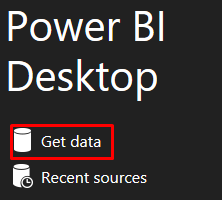
\includegraphics[scale=0.5]{./Imagenes/image001}
\item 3. En el cuadro de dialogo Obtener Datos (Get Data), click en base de datos SQL Server, y luego hacer click en Conectar (Connect) \\
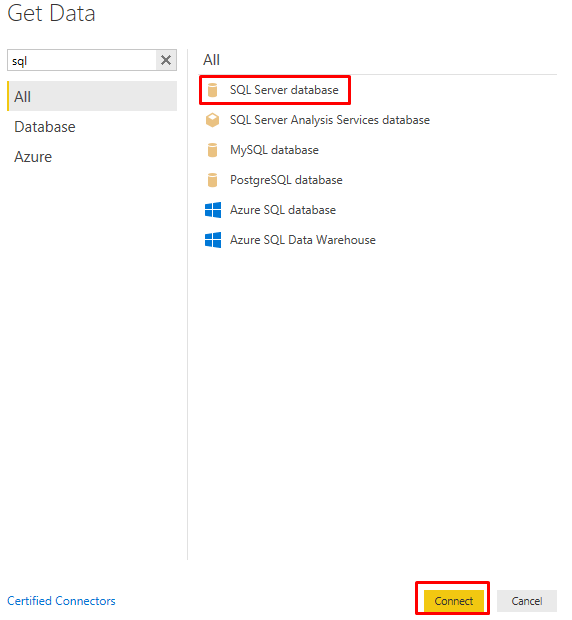
\includegraphics[scale=0.5]{./Imagenes/image002}
\item 4. En el cuadro de dialogo base de datos SQL Server, en la casilla servidor tipear (local), en la casilla Base de datos (opcional) / Database (optional), tipear AdventureWorks2017, y hacer clic en OK. \\
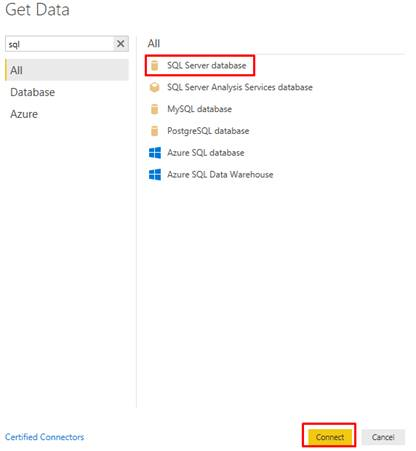
\includegraphics[scale=0.8]{./Imagenes/image003}
\item 5. En el cuadro de dialogo base de datos SQL Server, aceptar los valores por defecto, y luego click en el Conectar (Connect). Si un mensaje de Soporte de Encriptación es visualizado, hacer click en OK. \\
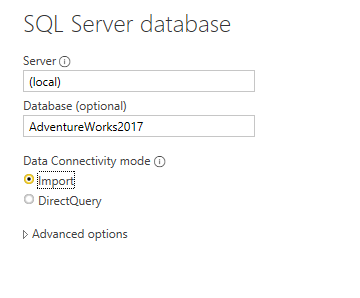
\includegraphics[scale=0.5]{./Imagenes/image004}
\item 6. En el cuadro de dialogo Navegador (Navigator), seleccionar el check en Sales.vSalesPerson, y entonces hacer click en Cargar (Load). \\
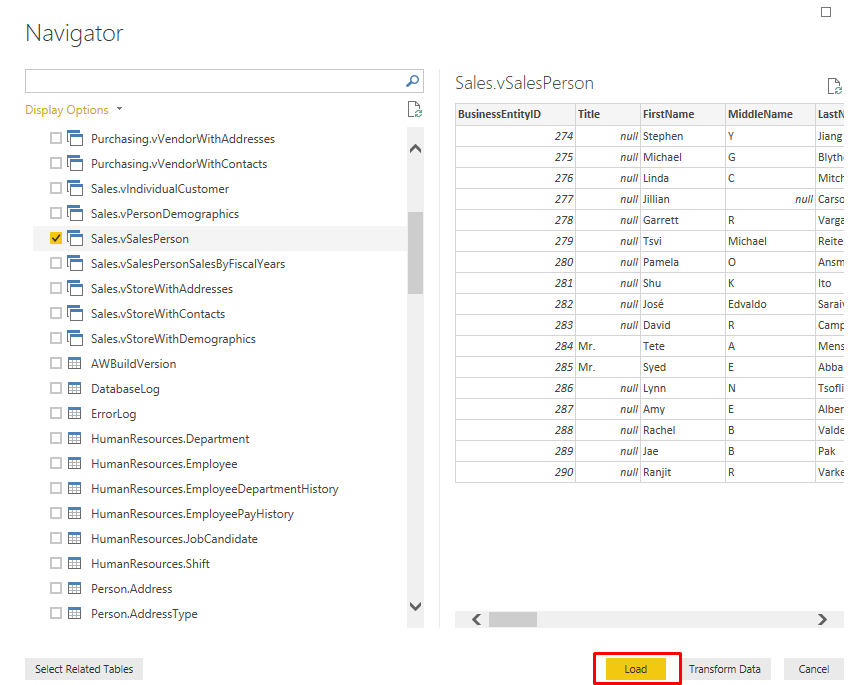
\includegraphics[scale=0.8]{./Imagenes/image005}
\item 7. En el panel Campos (Fields), expandir Sales vSalesPerson para ver todas las columnas. \\
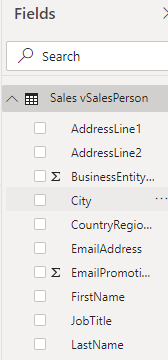
\includegraphics[scale=0.5]{./Imagenes/image006}
\item 8. En el menu principal (Home ribbon), hacer click en Funetes Recientes (Recent Sources), y en local: AdventureWorks2017. \\
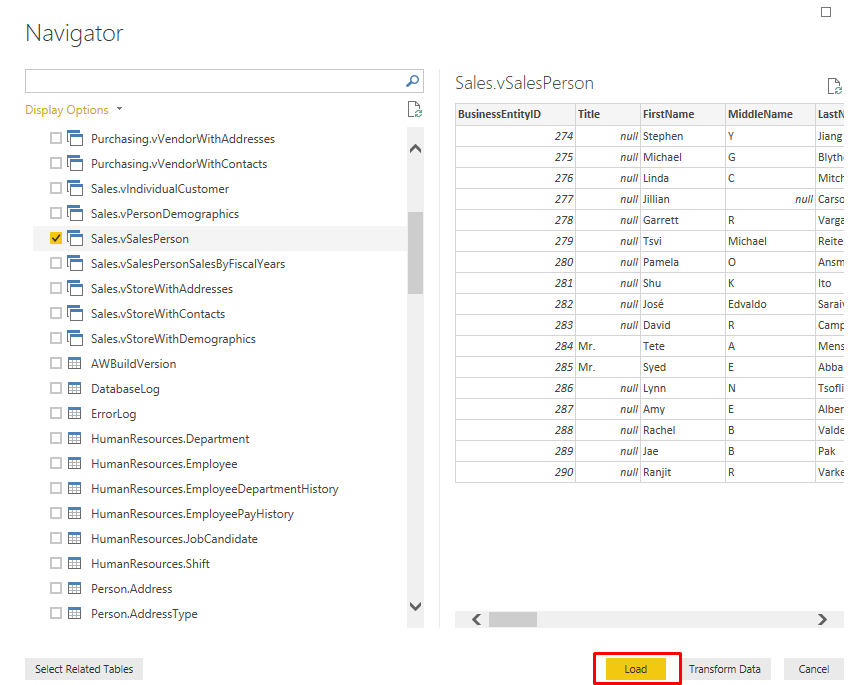
\includegraphics[scale=0.5]{./Imagenes/image007}
\item 9. En el cuadro de dialogo Navegador (Navigator), seleccionar la vista Sales.vStoreWithDemographics, y luego
hacer click en Cargar (Load). \\
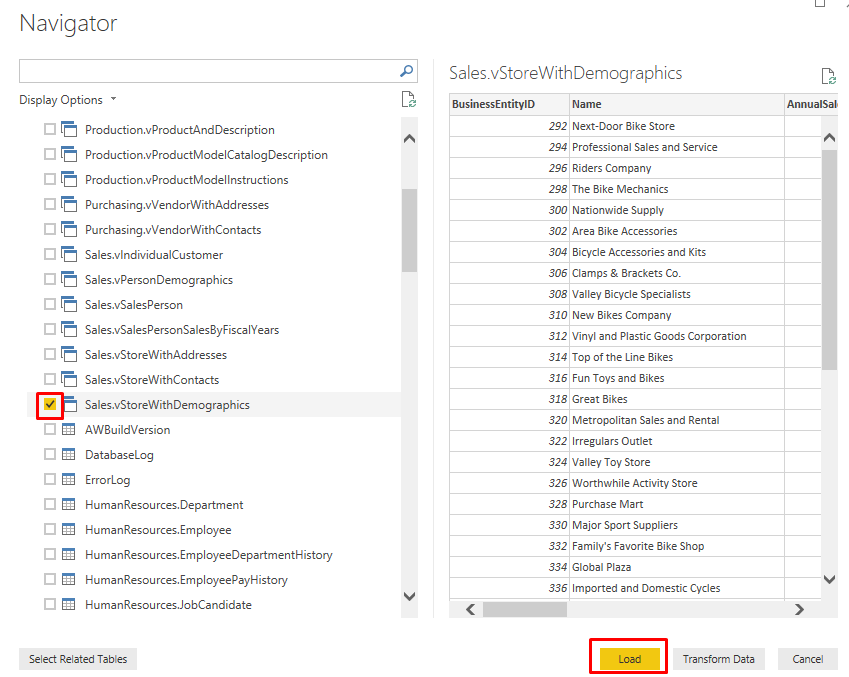
\includegraphics[scale=0.8]{./Imagenes/image008}
\item 10. En el panel Campos (Fields), expandir Sales.vStoreWithDemographics para ver todas las columnas. \\
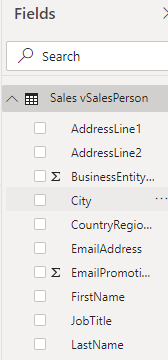
\includegraphics[scale=0.5]{./Imagenes/image009}
\item 11. En el menu principal (Home ribbon), hacer click en Obtener Datos (Get Data), y luego click en SQL Server. \\
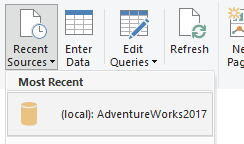
\includegraphics[scale=0.5]{./Imagenes/image010}
\item 12. En el cuadro dialogo base de datos SQL Server, en la casilla Servidor (Server), tipear (local), y en la casilla Base de datos (opcional), tipear AdventureWorks2017. \\
\item 13. Expandir opciones Avanzadas, en la casilla sentencia SQL (opcional, base de datos requerida), tipear la siguiente consulta, y luego hacer click en OK:
\\ SELECT TOP 10 P.ProductID, P.Name AS Product, SUM(CAST(LineTotal AS decimal(18,2))) AS LineTotal FROM
 Purchasing.PurchaseOrderDetail AS POD INNER JOIN Production.Product AS P ON POD.ProductID = P.ProductID \\
GROUP BY P.ProductID, P.Name ORDER BY LineTotal DESC \\ 
\item 14. Si la Ventana Configuración de la Conexión (Connection Settings) aparece, hacer click en OK. \\
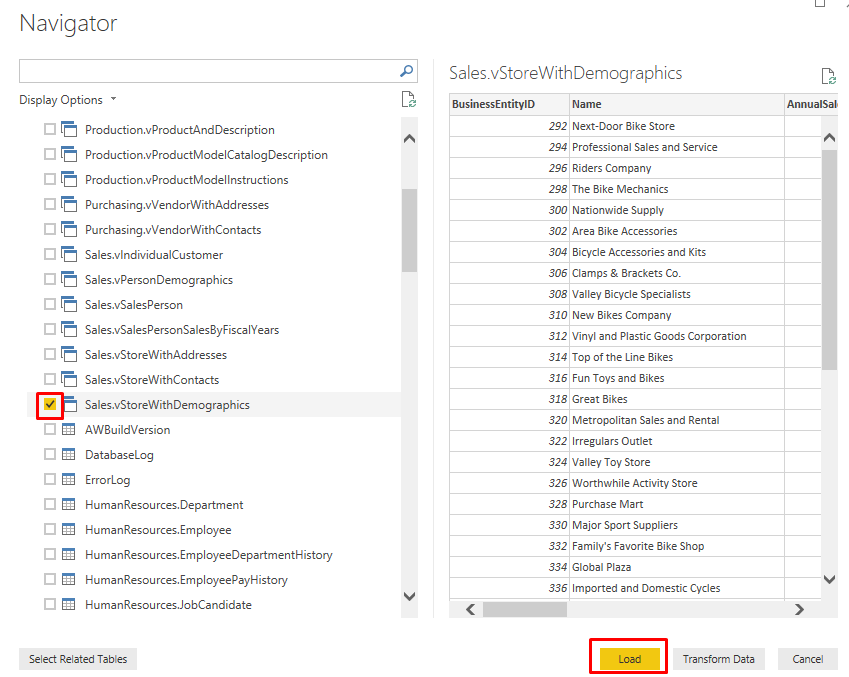
\includegraphics[scale=0.5]{./Imagenes/image011}
\item 15. En el cuadro de dialogo (local): AdventureWorks2017 hacer click en Cargar (Load). \\
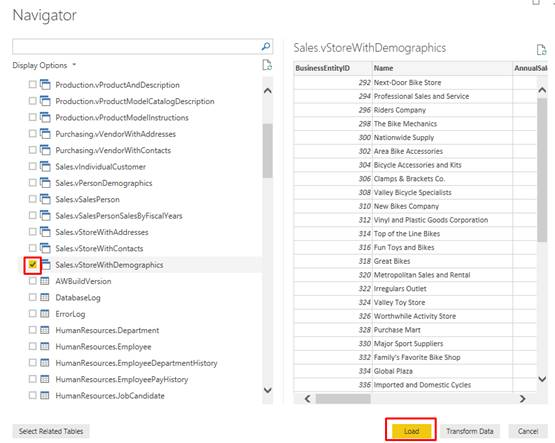
\includegraphics[scale=0.8]{./Imagenes/image012}
\item 16. En el panel Campos, expander Query1 para ver todas las columnas. \\
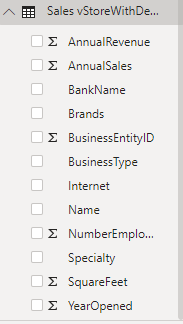
\includegraphics[scale=0.5]{./Imagenes/image013}
\item 17. Hacer click en la elipsis (…) al lado de Query1 y hacer click en Renombrar, tipear Top 10 Producto Vendidos, y presionar Enter. \\
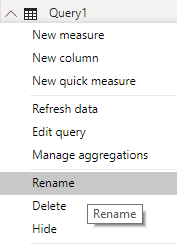
\includegraphics[scale=0.5]{./Imagenes/image014}


\end{itemize}
\section{ADICIONAR GRAFICOS AL REPORTE} 

\begin{itemize}

\item 1. En el panel Visualizaciones (Visualizations), hacer click en el gráfico Columna apilada (Stacked column) para
añadir el control al reporte. \\
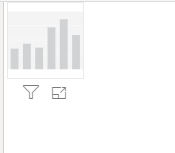
\includegraphics[scale=0.5]{./Imagenes/image015}
\item 2. En el panel Campos (Fields), bajo Sales vSalesPerson, arrastrar el campo FirstName a la casilla Eje (Axis) en el
panel de Visualización (Visualizations). \\
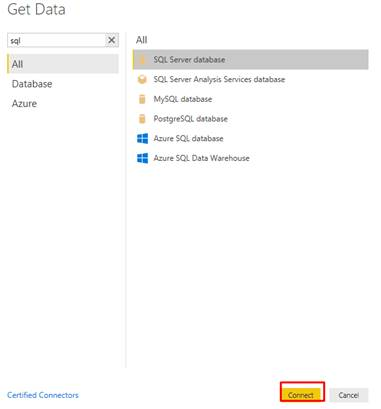
\includegraphics[scale=0.5]{./Imagenes/image016}

\item 3. Arrastrar el campo SalesYTD a la casilla Valores (Values). El gráfico se llenará con datos.\\
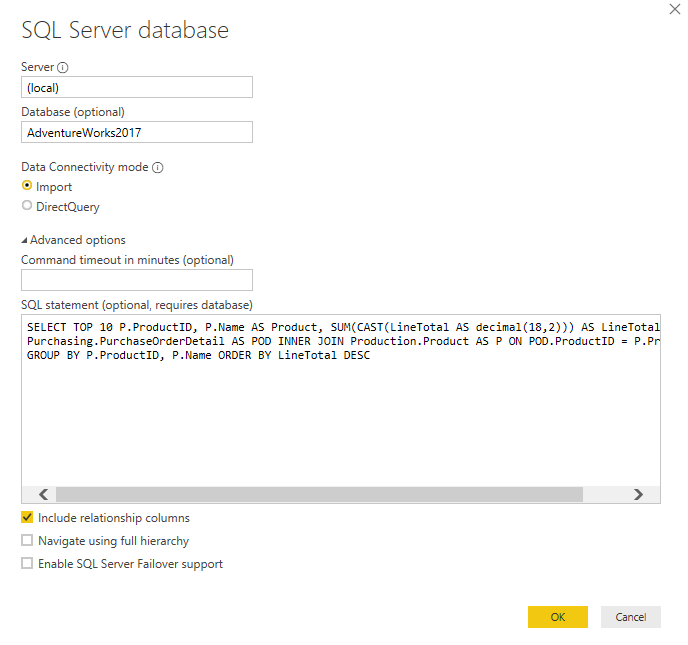
\includegraphics[scale=0.5]{./Imagenes/image017}
\item 4. En el gráfico en el reporte, ajustar el tamaño del gráfico para que muestre a todo el personal de ventas. \\

\includegraphics[scale=0.5]{./Imagenes/image018}
\item 5. Asegurarse que el gráfico tiene el foco y luego ir al panel de Visualización (Visualizations), hacer click en la pestaña Formato (Format). \\
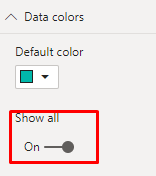
\includegraphics[scale=0.5]{./Imagenes/image019}

\item 6. Expandir Colores de datos (Data colors), activar la opción Mostrar todos (Show all). \\
\item 7. Cambiar el color para Jae, Linda, y Michael a rojo. \\
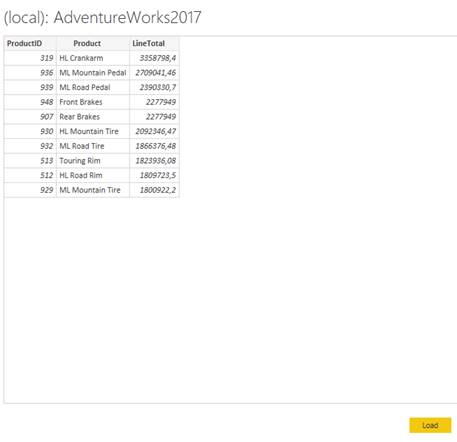
\includegraphics[scale=0.5]{./Imagenes/image020}
\item 8. Hacer click en el área de reporte y luego en el panel de Visualizaciones (Visualizations pane), hacer clic en el gráfico Pie para añadir el control al reporte. Arrastrar el gráfico Pie al lado derecho del gráfico de barras o debajo si no hubiese espacio.  \\
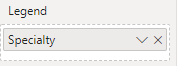
\includegraphics[scale=0.5]{./Imagenes/image021}
\item 9. En el panel Campos (Fields pane), bajo Sales vStoreWithDemographics, arrastrar el campo Specialty a la casilla Leyenda (Legend) en el panel de Visualizaciones. \\
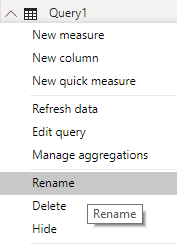
\includegraphics[scale=0.5]{./Imagenes/image022}

\item 10. Arrastrar el campo NumberEmployees a la casilla Valores (Values). El gráfico se llenará con los datos y mostrará tres secciones. \\
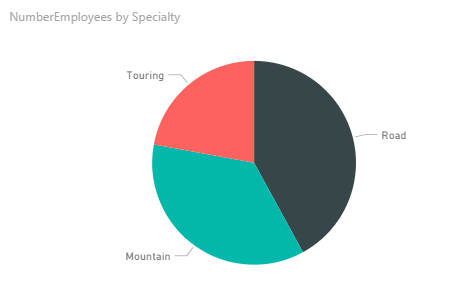
\includegraphics[scale=0.5]{./Imagenes/image023}
\item 11. Nuevamente click en el área de reporte, luego ir al panel de Visualizaciones y añadir otro gráfico de Columna apilada (Stacked columna) al reporte. Este gráico debe estar debajo de los gráficos previos. \\
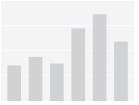
\includegraphics[scale=0.5]{./Imagenes/image024}

\item 12. En el panel Campos, expander Top 10 Productos Vendidos, arrastrar el campo Product a la casilla Eje (Axis) en el panel de Visualizaciones. \\

\item 13. Arrastrar el campo LineTotal a la casilla Valores (Value). El gráfico se llenara con datos. \\
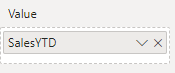
\includegraphics[scale=0.5]{./Imagenes/image025}

\item 14. Hacer click en el gráfico Top 10 Productos vendidos, entonces en el Panel de Visualizaciones, hacer click en el gráfico Donut. Revisar que fácil alternar un tipo de gráfico diferente. \\
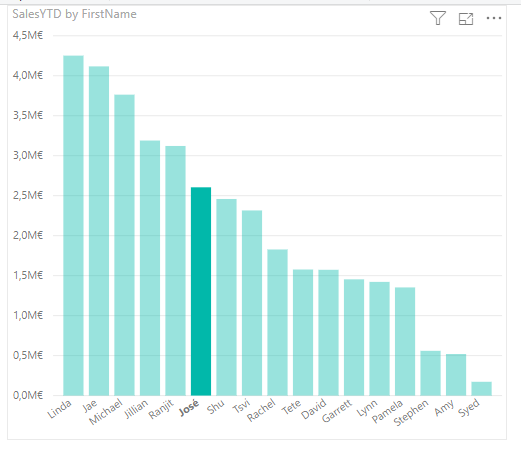
\includegraphics[scale=0.5]{./Imagenes/image026}

\item 15. En el gráfico, ajustar el tamaño para que se puedan visualizer todos los nombres de productos en el gráfico de Donut. \\

\item 16. En el panel Campos, bajo Sales vStoreWithDemographics, hacer click y arrastrar el campo AnnualSales directamente al área de reportes. Verificar como se crea automaticamente un gráfico de barras. \\

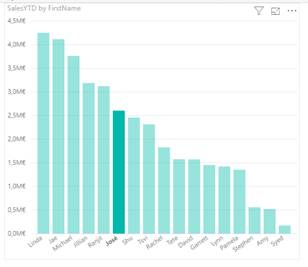
\includegraphics[scale=0.5]{./Imagenes/image027}

\item 17. En el panel Campos, seleccionar la casilla de verificación de AnnualRevenue, y apreciar que este adiciona el campo al gráfico de barras \\
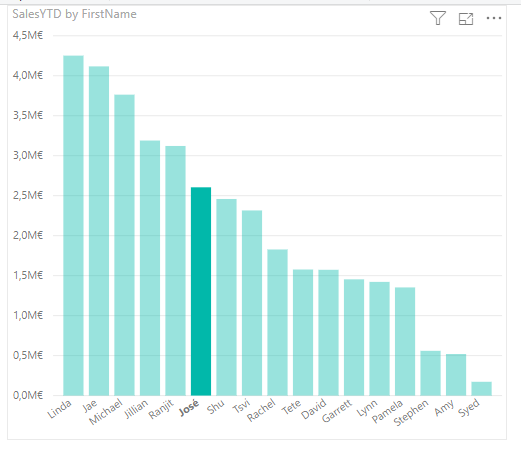
\includegraphics[scale=0.5]{./Imagenes/image026}
\item 18. En el panel Campos, hacer click en la elipsis (…) contigua a AnnualRevenue, y hacer click en Renombrar (Rename). Tipear Beneficios anuales luego presionar Enter. \\

\item 19. Repetir el paso 18, para renombrar el campo AnnualSales a Ventas Anuales. Apreciar que los nombres en los titulus y leyenda del gráfico de barras se han actualizado. \\

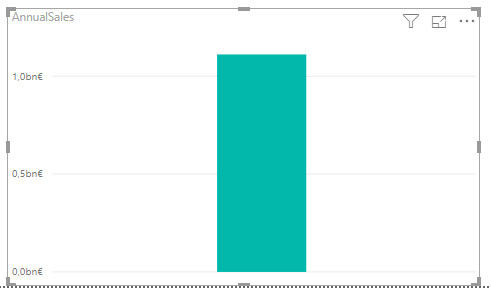
\includegraphics[scale=0.5]{./Imagenes/image028}

\item 20. Hacer click en el área de reporte, luego en el panel de Visualizaciones y en la pestaña Formato (Format). \\
\item 21. Expandir la Información de página (Page Information), y en la casilla Nombre tipear Ventas. Hacer click en el área de reporte y apreciar que el nombre ha cambiado en la pestaña al final del reporte. \\

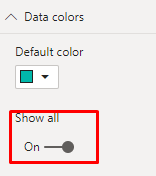
\includegraphics[scale=0.5]{./Imagenes/image029}

\item 22. En el menu Archivo (File menu), hacer click en Guardar (Save), crear un directorio Power BI, y guardar el archive como Ventas de Adventure Works Sales. \\

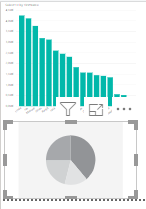
\includegraphics[scale=0.5]{./Imagenes/image030}



\end{itemize}


\end{document}
